\section{La température qui monte (3 points)}\label{ex:fusion}

Dans un récipient qui contient de l'eau, on a placé un thermomètre. On a relevé la température de l'eau toutes les 10 min.

\begin{center}
	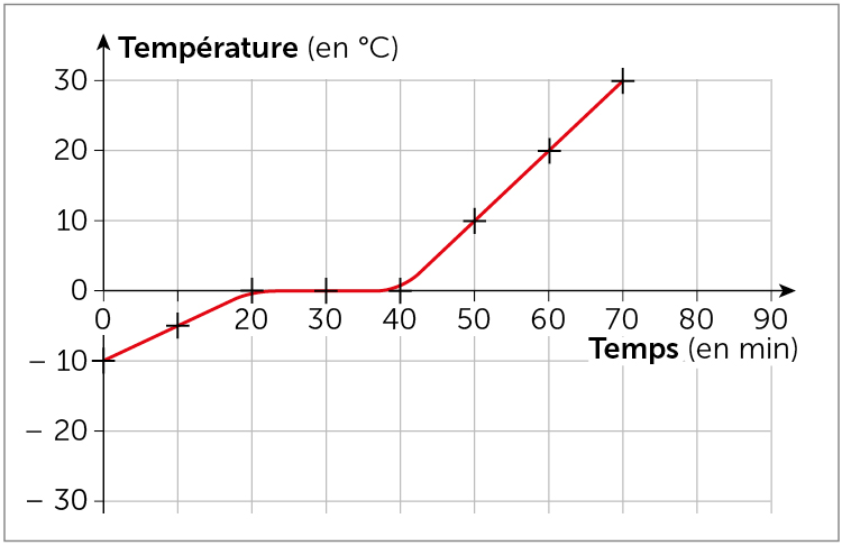
\includegraphics[scale=0.4]{./img/courbe}
\end{center}

\begin{questions}
	\question[1] Quel est l'état de l'eau après 10 minutes ? Après 60 minutes ?
	
	\question[1] Combien de temps a duré le changement d'état ?
	
	\question[1] A quel instant n'y a-t-il plus d'eau solide dans le récipient. 
\end{questions}